%
% File: chap01.tex
%
\let\textcircled=\pgftextcircled
\chapter{Introduction}
\label{Chapter1}
%This chapter provides the reader the necessary information to get familiar with the present work. It intends to contextualize the reader with the topics in the subsequent chapters and show them the path that should be followed.

\section{Presentation}
Combinatorial Optimization is a prominent field that results from the intersection of mathematics and theoretical computer science, specifically from areas such as combinatorics, algorithm theory, and operations research. Combinatorial Optimization problems are characterized by their solution space that consists of a finite collection of objects. This collection of objects typically grows exponentially in size, so going through all the objects and selecting the optimal one is not feasible~\cite{schrijver-book}.

The computational complexity behind solving Combinatorial Optimization (CO) problems is a very well-known concern, but the main motivation to solving them is the number of real-life problems that can be modeled using this framework. Thus, developing new techniques that provide Combinatorial Optimization algorithms which perform well has been in the spotlight for more than 50 years~\cite{appcombinatorial}, and it is the subject matter of this research.

% Check this citation
Considering the aforementioned, it is important to note what the essence of a CO algorithm is. As explained eloquently by Maltby and Ross~\cite{brilliant}, a CO algorithm uses mathematical methods either to make the search of possible solutions faster or to reduce the size of the set of feasible solutions. Some of the state-of-the-art techniques that have been proposed to produce those algorithms can be summarized as:

\begin{itemize}
\item Heuristic methods: a series of strategies where experience-based techniques are followed to solve the problem. Generally used when classical methods are too slow and when an approximate solution is enough for the implicit purposes.%~\cite{heuristics}
\item Branch and bound method: consists of a systematic division of the solution space where the core elements are called \textit{branches}. Then, branches are recursively explored and compared against estimated bounds of the optimal solution. \cite{branchbound}
\item Mixed/Integer Programming: some of the decision variables in the problem are constrained to be integer values at the optimal solution, and then, the problem can be solved by one or several methods before mentioned.
\end{itemize}

\begin{figure}[h!]
    \centering
    \label{fig:branchbound}
    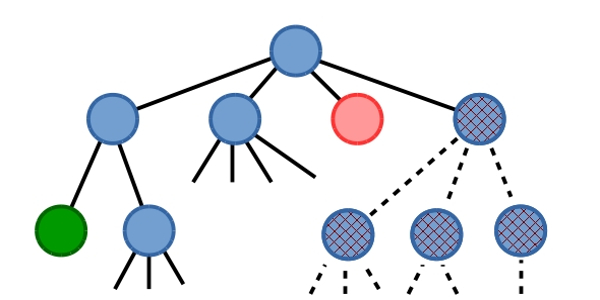
\includegraphics[scale=0.5]{theory_branch_and_bound.jpg}
    \caption{Illustration of the process of solving a CO algorithm with the branch and bound method~\cite{branchimage}.}
\end{figure}

For further information about the most popular strategies or an exhaustive explanation of those techniques, those considered to be good resources are~\cite{fernandes} and~\cite{integeroptimization}.

It is well known that most CO problems can be modeled with mathematical graphs~\citep{appcombinatorial}. Hence, most of the efforts in developing CO algorithms are dedicated to solving graph problems. These efforts have incremented in the last decade on account of the rapid growth in digital technology. Along with this change, the computing needs and the usual assumptions that algorithms used to make have become more demanding in terms of resource allocation.

%% proposals
%% imply
%% thesaurus for synonyms
On one hand, there is a need to research new theoretical proposals and to further investigate the new constraints that modern problems imply. Then, one could use this knowledge to influence the way new strategies approach those problems. On the other hand, there is a pragmatic need to solve those problems in real life and come up with practical and efficient solutions in a considerably small amount of time. In short, the theoretical and practical aspects need to be considered as part of the equation in contemporary applications where strong optimization strategies, like heuristic methods and Integer Programming, are just not enough.

%%%%% Reviewed until here %%%%

The ability to address the underlying issues that arise in this kind of problems has been improved drastically during the last years. Those huge steps are directed to obtain fast approximations for CO problems and have given rise to new ways to find algorithms that provide empirical efficient solutions.

Some recent approaches are being designed to take advantage of Machine Learning capabilities. In particular, Deep Learning strategies are providing alternative ways to deal with some of the underlying issues that arise with those kinds of problems. For determined problems, those approaches have shown to be the most successful in terms of running time efficiency, less human intervention, and the quality of the solutions.

Balanced graph partitioning is one of the fundamental Combinatorial Optimization problems and one of those who has gotten the best from Deep Learning. In simple words, the Balanced Graph Partitioning Problem is the task of finding a partition of a given graph into mutually exclusive sub-graphs, i.e. they do not share nodes, such as the partitions have the same size relative to the given measure. Finding a partition with the desired characteristics is a hard task, but the importance of solving it due to its numerous applications has incremented in recent years.

\section{Objectives}

\subsection{General objective}
    The main target of this research is to developing a machine learning algorithm that solves the graph partitioning problem that is capable of performing on abstract graphs and large-scale graph instances.
\subsection{Particular objectives}
The following objectives are the relevant expected goals to accomplish with this research:
\begin{itemize}
    \item To understand and analyze the Generalizable Approximate Partitioning (GAP) framework and to use it for solving the graph partitioning problem.
    \item Based on GAP, design an algorithm that works for general (non-attributed) graphs and at the same time relies completely on their structure.
    \item To build a framework that is easy to modify in order to use different objective functions in the partitioning stage.
    \item To explore different types of sampling and study the impact they have in the efficiency of the algorithm.
\end{itemize}
\section{Justification}

Graphs are a mathematical representation of what is colloquially known as networks. They are used to describe the relationships between objects which is adopted as a similitude measure and allows to model an extensive amount of real life problems. Due to their modeling capacity and their power of abstraction, they are widely studied in different areas of computer science and applied mathematics. 

The Graph Partitioning (GP) problem is relevant to solve a big number of graph-related tasks. Frequently, GP is employed as a pre-processing subroutine to solve a separate graph-related problem. If the edges that cross between the partition groups is relatively small compared to the original graph, then the partitioned graph may be better appropriate for analysis and problem-solving than the original~\cite{bettersuited}. 

As a matter of fact, finding good quality partitions of a graph is generally the first step of distributed graph computing tasks. The next paragraphs are dedicated to describe some of the most distinguished applications of GP.
Applications of GP into solve graph-related and other abstract computer science problems are presented first to continue then with applications to other areas and real-life situations.

One of the first and most useful applications of GP that one can find in literature is graph compression. A popular method for graph compression is the reordering method, which iteratively bisects a graph into two sets of equal cardinality aiming to minimize a compression-related objective function. Note that graph bisection is a special case of GP.\\ For instance, Bouritsas et. al.~\cite{compressgraphs} showed a way to use a Machine Learning approach combined with a parametric GP algorithm to solve this task.

Another important application of GP is to implement graph sparsification and related to this solving linear systems~\cite{sparcification}. In its paper, Gupta~\cite{matrixordering}

Nested dissection a divide and conquer heuristic for the solution of sparse symmetric systems of linear equations~\cite{nesteddissection}

A close-related 
Applications of graph partitioning to real-life problems:

Graph partitioning plays an essential role in paralleling computations and the design of new algorithms on large graphs. For example device placement problem where one aims to distribute work accross multiple devices and have applications in Deep Learning to train Neural Networks accross multiple devices \cite{deviceplacement} 

problem of intentional islanding in power systems considering load generation balance ~\cite{islanding}

Image segmentation~\cite{imagesegmentation}

communities detection
With

Undoubtedly, the most recent direction where the GP problem has gained importance is in its application for clustering in complex networks. Those types of networks include but are not limited to social networks, transportation networks, web graphs, and biological networks. For an example, see Figure~\ref{fig:complexnetwork}.

\begin{figure}[h!]
    \centering
    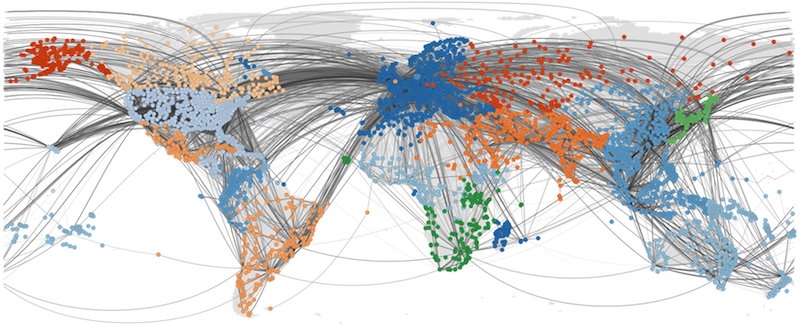
\includegraphics[scale=0.5]{complex_networks.png}
    \caption{The global mobility network. Representation of 4069 airports worldwide where gray lines between them are direct connections \cite{complexnetworks}.}
    \label{fig:complexnetwork}
\end{figure}

Most of the mentioned research and applications have in common that the approaches followed regularly use state-of-the-art GP algorithms. Some of the same algorithms for those tasks are unexplored in large-scale graphs and they do not consider the growth in instance-size of graph data that is emerging. The possibility that they become obsolete in the near future needs to be studied carefully as the same time alongside with the development of new strategies that overcome the inexorable challenges.

Another important highlight he targets are load-balance and minimizing the communication volume. This is a consideration not all of the existing approaches have.

\section{Project scope and limitations}
During the development of this project there were taken the following considerations
\begin{itemize}
    \item One of the first limitation found is related to the dataset used to test the proposed algorithm. Most of them were taken from "The Graph Partitioning Archive", a famous dataset where some of the most successful partitioning algorithms have been tested. While this offers a good comparison point, the algorithm have not been tested on real-world graphs.
    \item Again, due to the use of "The Graph Partitioning Archive" as dataset, the size of the graphs is not so big compared to real-world graphs as the ones used in Amazon or Pinterest networks. The largest graph in the dataset contains $500,000$ nodes.
    \item In general, the graphs used for running the experiments are not so sparse. Some of the graphs that are indeed sparse, belongs to the category of small-size graphs with less than $50,000$ nodes. This is not supposed to be a big deal because not all real-world graphs are sparse. However, it is believed that special considerations should be contemplated during the training of the algorithm.
    \item Most of the parameters values based on previous work where they were shown to have a good performance or they were recommended by the original authors. Nonetheless, more experiments in different scenarios should be run to determine better specific-task values.
    \item The machines where the experiments were executed have very limited power computing relative to the ambitions of this project. Though hardware specification of those machines was enough to run experiments on the selected dataset, it would be impossible to process complex networks with this technology.
    \item The proposed algorithm was not designed to run in a distributed environment. Experiments were run in single thread and the algorithm was trained only in GPU. Modifications of the algorithm to run in parallel and distribute the training load between CPU and CPU could be interesting to research topic and would improve its performance.
    \item The proposed framework only accepts certain input formats for the graphs, more specific JOSTLE and METIS formats.
    %\item Comparison with GAP was using graphs without features, an interesting thing would be to check performance with the same datasets they used but getting rid of the features, e.g., cora citation
\end{itemize}

\section{Research Problem}
The state-of-the-art algorithms for graph partitioning 
Graph partitioning algorithms based on DL

https://arxiv.org/pdf/2104.03546.pdf
\section{Hypothesis}
When analyzing GAP in depth some observations were made.

\section{Project organization}

